\subsection{The Motivation}

Our goal when we integrate a function is to find the amount of `space' between the graph and x-axis (or the Abscissa if you're fancy - but I'll just say x-axis). It's difficult to say how much space an arbitrary curve takes up, but we can work out the area of rectangles very easily - by calculating the {\em base $\times$ height}. Riemann integration takes advantage of this, and defines the integral of a function $f:\R \rightarrow \R$ by first bounding it from above with rectangular functions and finding a lower bound, then bounding it from below and finding an upper bound, then hoping that these two limits match up. 

\begin{figure}[H]
\centering
\begin{minipage}{.5\textwidth}
  \centering
  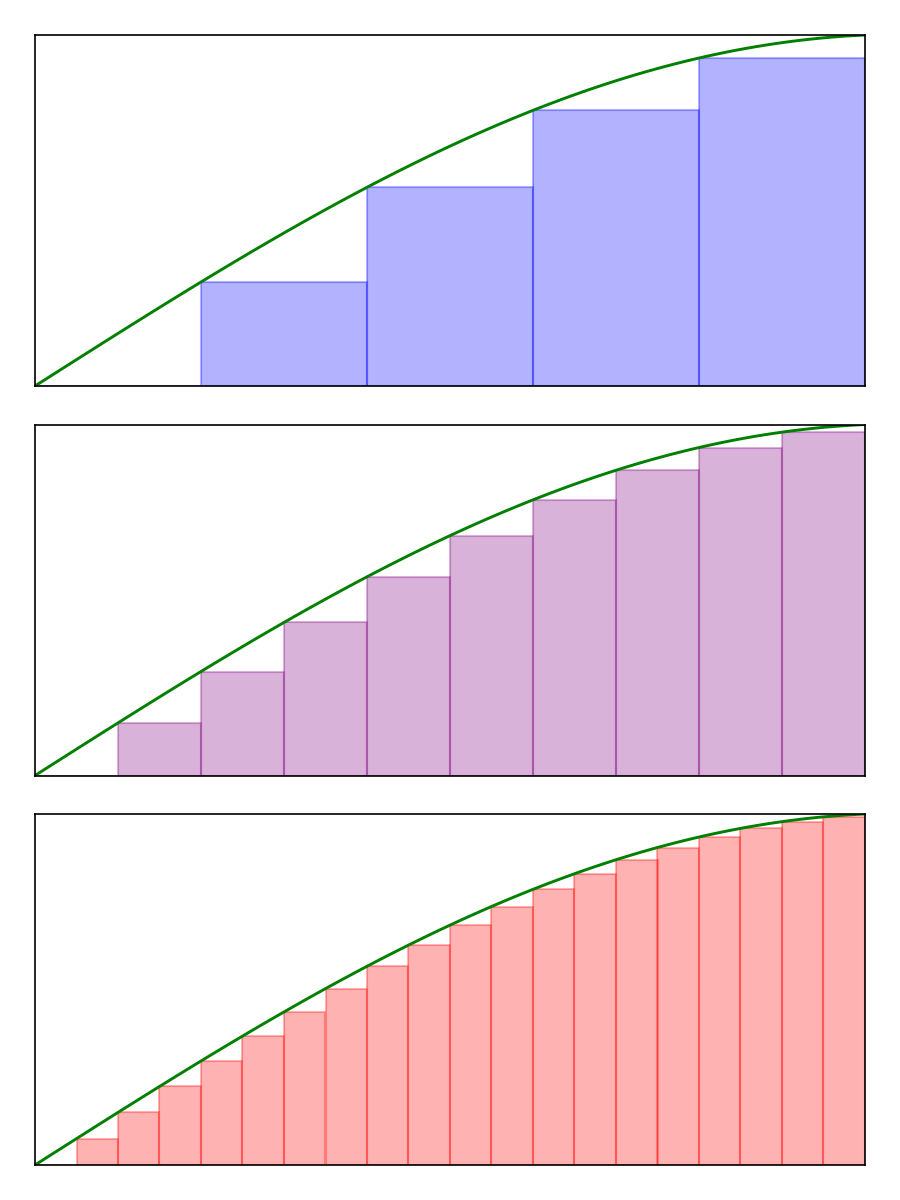
\includegraphics[scale=0.5]{Code/Area1.png}
  \captionof{figure}{Bounding from Below}
  \label{fig:test1}
\end{minipage}%
\begin{minipage}{.5\textwidth}
  \centering
  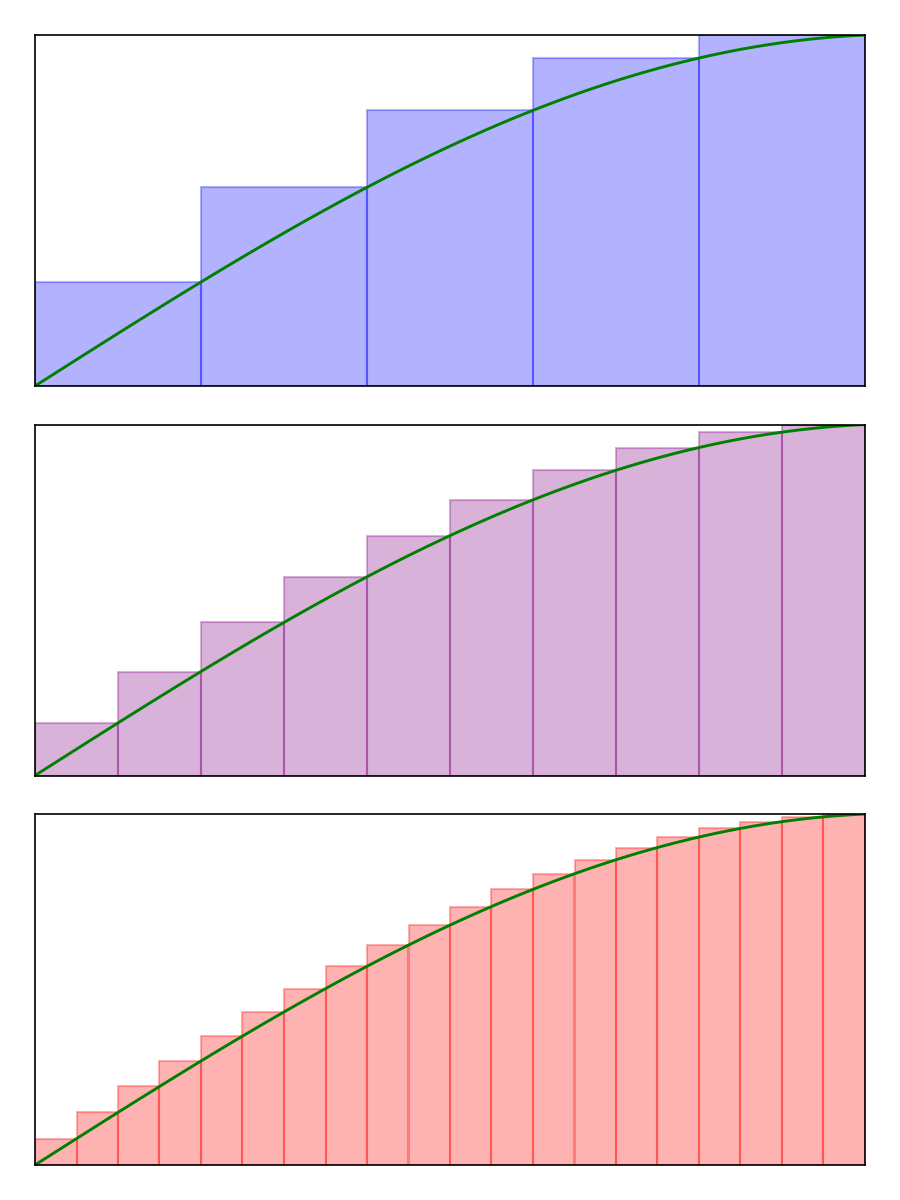
\includegraphics[scale=0.5]{Code/Area2.png}
  \captionof{figure}{Bounding from Above}
  \label{fig:test1}
\end{minipage}
\end{figure}

If the domain of our function (the `x-axis'), is $\R^2$ instead of just $\R$, we'd actually calculating a volume by finding the `space' between the graph and the axis. Basic Riemann integration doesn't apply to these functions - still, you can think of the `area of a rectangle' (which in this case would be the volume of a cuboid) as being calculated in much the same way; the size of the base (which is now an area, instead of a length) $\times$ the height.

With this is mind, lets clear up some of the terms we are going to use:

{\bf \em Lebesgue integration\/} is the method of integration defined above. Just like Riemann Integration, it is used to find the space between the graph of a function and the domain. However, unlike Riemann, the domain can be any set at all. Thinking back to rectangles and cuboids and $base \times height$, if we wanted make sense of what it means for there to be space between the graph and the x-axis, we should be able to make sense of the `size' of parts of the domain, so that we can figure out how big our base is and multiply that by the height$\ldots$

{\bf \em The Lebesgue Measure\/} seems then like it'd be a way to assign sizes to, or `measure' sets in the domain; but it is not! It's used specifically when we give sizes to the subsets of $\R^n$, and those sizes (or `measures') coincided with our usual idea of the size of a set in $\R^n$ - i.e. it is used when we are considering functions $\R^n \supset Y \rightarrow \R$, and in $\R$ the measure (length) of the interval $[1, 0]$ is 1, in $\R^2$ the measure (area) of the rectangle $[1, 0] \times [1, 0]$ is 1, in $\R^3$ the measure (volume) of the cube $[1, 0] \times [1, 0] \times [1, 0]$ is 1$\ldots$ etc. 

{\bf \em The Lebesgue Integral\/} is what we get when we do Lebesgue Integration on a set with the Lebesgue Measure on it. i.e. it's the intergral of functions $\R^n \supset Y \rightarrow \R$. This is the (basically) the same domain as the Riemann integral and so we'd want to check that these two things match up - and then see if the Lebesgue integral is better in some way.

To see the motivation behind the Lebesgue integral over Riemann, let's look at the canonical example of a function for which the Riemann integral fails; $f:\R \rightarrow \R,\ \ f(x) = \mathbbm{1}_\Q(x)$.

*Picture of this function*

First, let's define the Riemann integral. The definition of the Riemann integral involves many steps, and so it's quite long.
First, lets give the definition of a step function;
\begin{definition}{{(\em Riemann Integration\/})}
	Given;
	\begin{itemize}
		\item A function, $f: \ \R \rightarrow \R$
		\item A
	\end{itemize}
\end{definition}
	



